\chapter{Experiments\label{cha:chapter5}}

\section{Description of the Data Set\label{sec:dataset}}
The dataset used in this thesis is the HySpecNet-11k dataset developed by Fuchs et.al. \citep{fuchs_hyspecnet-11k_2023}. HySpecNet-11k is a hyperspectral benchmark dataset that consists of 11,483 image patches containing large-scale views of the surface of the earth. The image patches do not overlap which is advantageous for use in learning-based approaches as there are no duplicated image parts in the training set. The source data for the dataset uses 224 spectral bands and $128\times 128$ pixels spatially with a \ac{gsd} of 30 meters. However, we use the preprocessed version of the dataset which removes 20 spectral bands due to high water vapor absorption in those bands. We therefore only use 202 spectral bands. The image patches are of high quality because the tiles they were obtained from contain less than 10\% snow and cloud cover and were radiometrically, geometrically and atmospherically corrected \citep{fuchs_hyspecnet-11k_2023}. Furthermore, cropped patches at the borders of tiles were discarded, so each image patch contains information in all $128\times 128$ pixels. For splitting the dataset into training, validation and test set we used the provided patch-wise splitting set. This means that patches from the same tile can be present in different sets, unlike in the tile-wise splitting set. We did not perform experiments with the tile-wise splitting set as it is outside of the scope of this thesis. It is however an interesting research direction for the future.

\section{Loss Functions and Metrics}

\subsection{MSE Loss}
The \ac{mse} function is a common loss function used for training \acp{ann}. For the task of compressing a hyperspectral image it can be defined as follows:
\begin{align}
\text{MSE}(X,\hat{X}) = \frac{1}{B*C*H*W} \sum_{b=1}^{B}\sum_{c=1}^{C}\sum_{h=1}^H\sum_{w=1}^W (x_{bchw} - \hat{x}_{bchw})^2
\end{align}
Here $X$ is defined as a batch of hyperspectral input images, $\hat{X}$ the reconstruction of the images in $X$ obtained from the compression model, $B$ the number of images per batch and $C$,$H$ and $W$ the number of spectral channels, height and width of the hyperspectral images respectively.
We use \ac{mse} loss for pre-training the spectral autoencoder models as well as for training the \ac{cnn}-based spatial autoencoder outside of the combined model.

\subsection{Rate Distortion Loss}
In contrast to the purely \ac{cnn}-based models with a fixed compression rate for a given set of hyperparameters, the hyperprior-based models have a variable compression rate that changes during the training process. This comes from the fact that the bitrate of the arithmetic coder depends on the performance of the hyperprior \ac{cnn}. Because of this \ac{mse} loss is not optimal for these models. While it is possible to train hyperprior-based models using \ac{mse} loss because the bitrate dependency is contained in the lossless arithmetic coder, this leads to very high bitrates. However, using \ac{mse} loss for a hyperprior model can still be useful to obtain an upper bound on the reconstruction accuracy for a given set of hyperparameters. For more elaboration on this see TODO.

To train a model using an arithmetic coder in the bottleneck with both a low distortion and a low bitrate, a different loss function is needed. The type of problem that arises is a rate-distortion optimization problem \citep{balle_variational_2018}. This can problem can parametrized in the following way \citep{minnen_joint_2018}:
\begin{align}
R + \varphi \cdot D = \underbrace{\mathbf{E}_{x\sim p_x} [ -\log_2 p_{\hat{y}}(\lfloor f(x)\rceil)]}_\text{rate}+ \underbrace{\varphi \cdot\mathbf{E}_{x\sim p_x} [d(x,g(\lfloor f(x)\rceil))]}_\text{distortion}.
\end{align}
We parametrize the rate-distortion trade-off with the Lagrange multiplier $\varphi$. (We use $\varphi$ instead of the commonly used $\lambda$ to avoid confusion with the $\lambda$ of the \ac{dualmse} loss described in \autoref{sec:ch5dualmse}). $p_x$ is the unknown distribution of input images, $\lfloor\cdot\rceil$ refers to quantization and $f$ is the main encoder. Accordingly, $y=f(x)$ is the output of the main encoder applied to the input $x$, $\hat{y} = \lfloor y\rceil$ are the quantized latents of the main encoder, $p_{\hat{y}}$ is a discrete entropy model and $\hat{x}=g(\hat{y})$ is the reconstruction of $x$ obtained from applying the main decoder $g$ to the quantized latents $\hat{y}$. As the metric for computing the distortion we use \ac{mse}, because Ballé et.al. showed that the rate-distortion problem is equivalent to minimizing the \ac{kl} divergence over $p_x$ \citep{balle_variational_2018}. Using this equivalence they showed that using \ac{mse} as distortion metric is equivalent to assuming a Gaussian distribution for $p_{x|\hat{y}}(x|\hat{y})$. While there are approaches assuming different probability distributions like the Student's T distribution, this was not a focus of this thesis and the Gaussian often provides a good estimate for unknown probability distributions. For this reason we also assumed a Gaussian distribution for the probability distribution.

However, this formulation does not include the hyperprior network that learns and transmits side information about the entropy model $p_{\hat{y}}$. In order to incorporate the hyperprior into the \ac{rd} loss function, we need to add an additional term to capture the bitrate for the transmitted side information. The final loss function is then defined as follows:
\begin{align}
R + \varphi \cdot D &= \underbrace{\mathbf{E}_{x\sim p_x} [ -\log_2 p_{\hat{y}}(\lfloor f(x)\rceil)]}_\text{rate (main latents)} + 
\underbrace{\mathbf{E}_{x\sim p_x} [ -\log_2 p_{\hat{z}}(\lfloor f_h(f(x))\rceil)]}_\text{rate (hyper-latents)}\\ 
&\qquad\qquad\qquad\qquad\qquad\quad\:\: + \underbrace{\varphi \cdot\mathbf{E}_{x\sim p_x} [\Vert x - g(\lfloor f(x)\rceil))\Vert^2_2]}_\text{distortion}.\\
&=\underbrace{\mathbf{E}_{x\sim p_x} [ -\log_2 p_{\hat{y}}(\hat{y})]}_\text{rate (main latents)} + 
\underbrace{\mathbf{E}_{x\sim p_x} [ -\log_2 p_{\hat{z}}(\hat{z})]}_\text{rate (hyper-latents)} + \underbrace{\varphi \cdot\mathbf{E}_{x\sim p_x} [\Vert x - \hat{x}\Vert^2_2]}_\text{distortion}
\end{align}
Here $z$ and $\hat{z}$ refer to the latent of the hyperprior and the quantized latent of the hyperprior respectively, that being the result of applying both the main encoder $f$ and the hyperprior encoder $f_h$ to the input $x$.

With regard to the quantization operation, care has to be taken. When executing the trained hyperprior model, quantization is defined as rounding to the nearest integer. However, during training this would result in zero gradients everywhere. To avoid this, while training we instead apply a uniform noise to the input in place of rounding. From this follows that the arithmetic coder is only executed during testing, not during training. In training the achieved bitrate is estimated using a heuristic. However, we verified that the bitrate estimates are close to the real achieved bitrate in \autoref{sec:ch5heur}.
\subsection{Dual MSE Loss}
The combined model consists of an outer autoencoder model and an inner autoencoder model. However, applying a loss function such as \ac{mse} loss in the standard way results in the inner autoencoder being trained through a layer of distortion at both the input and the output, as the input to the loss function are the input to outer encoder $x$ and the output of the outer decoder $\hat{x}$. The input to the inner encoder, $y=f_o(x)$, where $f_o$ is the outer encoder and the output of the inner decoder, $\hat{y}=g_i(f_i(y))$, where $f_i$ and $g_i$ are the inner encoder and decoder respectively, are not direct inputs to the loss functions. To alleviate that, we designed an experimental loss function called \ac{dualmse} loss. It is defined as follows:
\begin{align}
\text{DualMSE}(x,\hat{x},y,\hat{y}) = \lambda * \text{MSE}(x,\hat{x}) + (1-\lambda) *  \text{MSE}(y,\hat{y}).
\end{align}
The \ac{dualmse} loss is therefore a linear interpolation between the \ac{mse} loss of the complete model and the \ac{mse} loss of the inner model. This allows for fine-grained control over the weight of the loss of the inner model in the overall loss. Of note are also the two edge cases of $\lambda = 1$, where the \ac{dualmse} loss function becomes equivalent to \ac{mse} loss and $\lambda = 0$, where only the loss of the inner model is used. The \ac{dualmse} loss was used for the combined models using the \ac{cnn}-based spatial autoencoder. Results regarding the use of \ac{dualmse} loss for these models can be seen in \autoref{sec:ch5dualmse}. While the use of a Dual Rate Distortion loss would be possible for the combined models using a hyperprior-based spatial autoencoder, this was not done because the results in \autoref{sec:ch5dualmse} did not show a clear and significant improvement when using a dual loss function.

\subsection{Metrics}
We use two different metrics to evaluate our experiments. The first metric is \ac{psnr}, which is a common metric to quantify reconstruction accuracy for lossy learning-based image compression \citep{balle_end--end_2017,balle_variational_2018,minnen_joint_2018,kuester_1d-convolutional_2021,kuester_transferability_2022,la_grassa_hyperspectral_2022}. \Ac{psnr}  is defined in general as follows:
\begin{align}
\text{PSNR}(x,\hat{x}) &= 10*\log_{10}\frac{\text{MAX}}{\text{MSE}(x,\hat{x})}
&= 20 * \log_{10}(\text{MAX}) - 10*\log_{10}(\text{MSE}(x,\hat{x})).
\end{align}
Here MAX is the maximum possible pixel value in the used dataset and $\text{MSE}(x,\hat{x})$ refers to the Mean Squared Error between $x$ and $\hat{x}$. However, since the data range for the HySpecNet-11k dataset used in this thesis is the intervall $[0,1]$, the equation simplifies to:
\begin{align}
\text{PSNR}(x,\hat{x}) = - 10*\log_{10}(\text{MSE}(x,\hat{x})).
\end{align}
It is therefore directly correlated with the log of the \ac{mse}.
While \ac{psnr} is a commonly used metric in lossy learning-based hyperspectral compression, it is computed as an average over all channels. We therefore want to employ another metric to more accurately evaluate the reconstruction of the spectral signatures which are important for lossy reconstructions of hyperspectral images.

For this we use the spectral angle. It is computed by calculating the angle between the spectra of the input image and the reconstruction for each pixel using the \ac{sam} algorithm \citep{kruse_spectral_1993}. The computed angles are then averaged to compute the metric for a given input image and reconstruction. Using the combination of \ac{psnr} and spectral angle we can compare different models with regard to spatial and spectral reconstruction accuracy.
\begin{table}
\centering
\begin{tabularx}{\textwidth}{|L|L|}
\hline
Model Name & Description \\
\hline\hline
Conv1D & Per-pixel spectral autoencoder (\autoref{sec:conv1d})\\
\hline
FastConv1D & \Ac{twod} spectral autoencoder (\autoref{sec:fastconv1d})\\
\hline
Conv2D & \Ac{twod} \ac{cnn}-based spatial autoencoder (\autoref{sec:conv2d})\\
\hline
AttentionHyperprior & Attention-based spatial model using hyperprior architecture (\autoref{sec:atthyperprior}) \\
\hline
Combined & Combined Model using Conv1D as the spectral part and Conv2D as spatial part (\autoref{sec:combinedmodel}) \\
\hline
FastCombined & Combined Model using FastConv1D as the spectral part and Conv2D as spatial part (\autoref{sec:combinedmodel}) \\
\hline
CombinedWithAttention & Combined Model using Conv1D as the spectral part and AttentionHyperprior as spatial part (\autoref{sec:combinedmodel}) \\
\hline
Spectral-VAE & Spectral \ac{vae}-based autoencoder (\autoref{sec:vae}) \\
\hline
\end{tabularx}
\label{fig:shortnames}
\caption{Shortnames for models}
\end{table}
\section{Impact of Hughes Phenomenon \label{sec:ch5hughes}}
\begin{figure}[!ht]
    \centering
\pgfplotstableread[col sep=semicolon,]{graphs/hughes.csv}\datatable
\begin{tikzpicture}
\begin{semilogxaxis}[
	log ticks with fixed point,
	grid=both,
    width=\textwidth,
    height=10cm,
    xtick=data,
    xticklabels from table={\datatable}{dsfactor},
    legend style={at={(0.98,0.3)},anchor=south east},
    ylabel={Psnr},
    xlabel={Division factor for dataset}]
    
    \addplot [mark=o, blue!80 ] table [x={dsfactor}, y={fastconv_psnr}]{\datatable};
    \addlegendentry{FastConv}
    
    \addplot [mark=o, red!80] table [x={dsfactor}, y={fastcombined_psnr}]{\datatable};
    \addlegendentry{FastCombined}
\end{semilogxaxis}
\end{tikzpicture}
\caption{Hughes Phenomenon combined vs fast combined}
\label{fig:hughes}
\end{figure}

\begin{figure}[!ht]
    \centering
\pgfplotstableread[col sep=semicolon,]{graphs/hughes.csv}\datatable
\begin{tikzpicture}
\begin{semilogxaxis}[
	log ticks with fixed point,
	grid=both,
    width=\textwidth,
    height=10cm,
    xtick=data,
    xticklabels from table={\datatable}{dsfactor},
    legend style={at={(0.98,0.3)},anchor=south east},
    ylabel={Spectral Angle},
    xlabel={Division factor for dataset}]
    
    \addplot [mark=o, blue!80 ] table [x={dsfactor}, y={fastconv_sangle}]{\datatable};
    \addlegendentry{FastConv}
    
    \addplot [mark=o, red!80] table [x={dsfactor}, y={fastcombined_sangle}]{\datatable};
    \addlegendentry{FastCombined}
\end{semilogxaxis}
\end{tikzpicture}
\caption{Hughes Phenomenon combined vs fast combined}
\label{fig:hughesangle}
\end{figure}

Hughes Phenomenon, also referred to as curse of dimensionality, describes the phenomenon that the number of required training samples for a learning-based algorithm is correlated with the dimensionality of the data \citep{hughes_mean_1968}. This is especially applicable to the domain of hyperspectral imaging because of the high number of spectral channels increasing the dimensionality of the input. We tested the impact of the Hughes Phenomenon on the \textbf{FastConv} model and the \textbf{FastCombined} model by varying the size of the training dataset. More details on the model labels is provided in \autoref{fig:shortnames}. All models in this experiment were trained using the Adam optimizer with the learning rate set to $0.5\cdot 10^{-4}$. The \textbf{FastConv} models were trained for 70 epochs, which resulted in convergence.
The trained \textbf{FastConv} models were then used as pretrained parts of the \textbf{FastCombined} models. The models were then trained for an additional 50 epochs using $\lambda=1$ while freezing the spectral encoder. 
The \textbf{FastConv} models used a compression ratio of 16 or a bitrate of 2 \ac{bpppc}. The FastCombined models used an additional spatial compression factor of 4, resulting in a total compression ratio of $16 \cdot 4=64$ or a bitrate of 0.5 \ac{bpppc}.

As seen in \autoref{fig:hughes} and \autoref{fig:hughesangle}, the models perform worse for smaller dataset sizes. However, for division factors $f < 8$ the gradient decreases with lower division factors, while between division factors 8 and 64 there is a high gradient in \ac{psnr} and spectral angle. A division factor of 8 on the HySpecNet-11k dataset results in 1004 training samples. Since the HySpecNet-11k dataset uses 202 spectral channels, we therefore require $1004/202 \approx 4.97$ training samples per channel until performance starts to decrease more quickly. Since for machine learning typically 5 training samples per dimension are recommended \citep{theodoridis_pattern_2009}, we conclude that our models are not especially strongly effected by the Hughes Phenomenon. However, while the improvement of the model achieved by increasing the dataset size is reduced for dataset sizes above this threshold, the metrics still achieve the best values when training on the complete dataset. For this reason we continued to use the full dataset for the following experiments.
\section{Dual MSE Loss Results And Latent Space Analysis \label{sec:ch5dualmse}}
\begin{figure}
	\centering
	\pgfplotstableread[col sep=semicolon,]{graphs/freezedualmse.csv}\datatable
	\begin{tikzpicture}
	\begin{axis}[
	    grid=both,
	    height=7cm,
	    width=\textwidth,
	    legend style={at={(0.95,0.1)},anchor=south east},
	    %legend to name={dualmselegend},
	    xtick={0,0.1,...,1},
	    ytick={20,25,30,35,40,45},
	    ylabel={Psnr (dB)},
	    xlabel={Dual MSE $\lambda$}]
	    
	    \addplot table [x={lmbda}, y={psnr_test}, 
	    restrict expr to domain={\thisrow{model_id}}{1:1}]{\datatable};
	    \addlegendentry{Combined-AllFrozen}
	    
	    \addplot table [x={lmbda}, y={psnr_test}, 
	    restrict expr to domain={\thisrow{model_id}}{2:2}]{\datatable};
	    \addlegendentry{Combined-EncoderFrozen}
	    
	    \addplot table [x={lmbda}, y={psnr_test}, 
	    restrict expr to domain={\thisrow{model_id}}{3:3}]{\datatable};
	    \addlegendentry{FastCombined-AllFrozen}
	    
	    \addplot table [x={lmbda}, y={psnr_test}, 
	    restrict expr to domain={\thisrow{model_id}}{4:4}]{\datatable};
	    \addlegendentry{FastCombined-EncoderFrozen}
	    
	    \addplot table [x={lmbda}, y={psnr_test}, 
	    restrict expr to domain={\thisrow{model_id}}{5:5}]{\datatable};
	    \addlegendentry{FastCombined-NothingFrozen}
	\end{axis}
	\end{tikzpicture}
	\caption{Dual MSE lambda plot}
	\label{fig:dualmselosspsnr}
	\end{figure}
For this experiment shown in \autoref{fig:dualmselosspsnr} we tested multiple different values for $\lambda$ in the \ac{dualmse} loss. The spectral angle values for this experiment are shown in \autoref{fig:dualmselossangle} in the appendix, as it shows similar results to \autoref{fig:dualmselosspsnr}. We did this for multiple variations of the Combined Model. All models in this experiment were trained using the Adam optimizer with the learning rate set to $0.5\cdot 10^{-4}$. All models were trained by first pretraining the spectral autoencoder for 70 epochs and then training the complete Combined Model for 50 epochs. Furthermore all models had a spectral downsampling factor of 16 and a spatial downsampling factor of 4, resulting in a total compression ratio of 64 or a bitrate of 0.5 \ac{bpppc}.

The tested models differ in two ways. Firstly, some models are of the \textbf{Combined} type while some are of the \textbf{FastCombined} type (see \autoref{fig:shortnames}). The other variable in which the models differ is whether the weights of the spectral autoencoder are frozen after pretraining. We tested freezing all weights after pretraining, making the complete model equivalent to training the spatial autoencoder while using the pretrained spectral encoder/decoder pair for pre- and postprocessing respectively. We also tested only freezing the weights of the spectral encoder after pretraining. In this way, the latent space produced by the spectral encoder does not change during training which we hoped could improve the training of the spatial autoencoder. Additionally, in contrast to the models where all weights of the spectral autoencoder are frozen after pretraining, the spectral decoder can still learn to adapt to the distortion introduced by the spatial autoencoder.

However, with the exception of $\lambda=0$ for the model where only the encoder is frozen after pretraining, no clear trends in the \ac{psnr} or spectral angle could be observed regarding the value of $\lambda$. However, regarding the decision on whether to freeze parts of the spectral autoencoder after pretraining it is valuable to freeze either the spectral encoder or the complete spectral autoencoder, since the \ac{psnr} of the model \textbf{FastCombined-NothingFrozen} is $1.5-2$ dB below the other \textbf{FastCombined} models for $\lambda = 0.5$ and $\lambda = 0.7$. For $\lambda=0$ \textbf{FastCombined-NothingFrozen} is much worse with a difference of over 20 dB. To analyse why the model \textbf{FastCombined-NothingFrozen} with $\lambda=0$ performed much worse than all other models, we computed the minimum and maximum values for the latent vectors $y$ of the spectral encoder and for the reconstructed latents $\hat{y}$ produced by the spatial autoencoder. For the model \textbf{FastCombined-EncoderFrozen} and \textbf{FastCombined-AllFrozen} these values behaved as expected with the maxima close to 1 and the minima close to 0. This is expected because the last layer of the spectral encoder is a sigmoid layer which constrains the latents to be in the interval $[0,1]$. However, for the model \textbf{FastCombined-NothingFrozen} both the minimum and the maximum approached 0.5. On the test set the minimum latent value was 0.4875 and the maximum 0.5118. The spatial autoencoder then reconstructed a constant output close to 0.5 for each channel. Because for $\lambda=0$ only the \ac{mse} between $y$ and the $\hat{y}$ is relevant, the model managed to minimize this loss by learning to reduce the distance of the inputs between the latents.

\begin{figure}
	\centering
	\pgfplotstableread[col sep=semicolon,]{graphs/freezedualmse.csv}\datatable
	\begin{tikzpicture}
	\begin{semilogyaxis}[
	    ymajorgrids=true,
	    xmajorgrids=true,
	    height=7cm,
	    xtick={0,0.1,...,1},
	    ytickten={-5,-4,-3,-2,-1},
	    width=\textwidth,
	    legend style={at={(0.5,0.6)},anchor=south east},
	    %legend to name={dualmselegend},
	    ylabel={Inner MSE Loss},
	    xlabel={Dual MSE $\lambda$}]
	    
	    \addplot table [x={lmbda}, y={inner_mse}, 
	    restrict expr to domain={\thisrow{model_id}}{3:3}]{\datatable};
	    \addlegendentry{FastCombined-AllFrozen}
	    
	    \addplot table [x={lmbda}, y={inner_mse}, 
	    restrict expr to domain={\thisrow{model_id}}{4:4}]{\datatable};
	    \addlegendentry{FastCombined-EncoderFrozen}
	    
	    \addplot table [x={lmbda}, y={inner_mse}, 
	    restrict expr to domain={\thisrow{model_id}}{5:5}]{\datatable};
	    \addlegendentry{FastCombined-NothingFrozen}
	\end{semilogyaxis}
	\end{tikzpicture}
	\caption{Inner mse plot}
	\label{fig:inner_mse}
	\end{figure}

However, while the usage of the \ac{dualmse} loss does not have a strong effect on \ac{psnr} or spectral angle with our models on the HySpecNet-11k dataset, it does succeed in strongly reducing the differences between the latent produced by the spectral encoder and its reconstruction. As shown in \autoref{fig:inner_mse}, using \ac{dualmse} loss with $\lambda < 1$ drastically reduces the inner \ac{mse}, which is the \ac{mse} between $y$ and $\hat{y}$. For \textbf{FastCombined-NothingFrozen} the inner \ac{mse} reduces from $0.133$ to $8.00\cdot 10^{-6}$, which is a factor of $\approx 16606$. For \textbf{FastCombined-EncoderFrozen} this factor is $\approx 1116$ and for \textbf{FastCombined-AllFrozen} the reduction factor is $\approx 196$, which are still large decreases in loss. This can also be seen visually when comparing the reconstructed latents as we have done in \autoref{fig:latentcompare}. We show the effect for \textbf{FastCombined-AllFrozen} since the frozen encoder gives the advantage of producing the same latent representations for all compared models, as the weights of the encoder are constant during training. It can be seen that with $\lambda=1$ the latents have a visible grid pattern that is not present when using $\lambda < 1$. A similar pattern can also be seen during the first epoch of training for models with $\lambda < 1$ and is therefore likely a result of the convolutional layers used in the \ac{twod} \ac{cnn}-based spatial autoencoder. During training these patterns disappear when the \ac{mse} between $y$ and $\hat{y}$ is part of the loss function, which is not the case for $\lambda=1$. However, the models with $\lambda=1$ produce similar overall reconstructions $\hat{x}$ as shown by the similar \ac{psnr} and spectral angle. The spectral decoder therefore is able to ignore these grid patterns even without additional training, since even the models \textbf{FastCombined-AllFrozen} and \textbf{Combined-AllFrozen} with $\lambda=1$ have a high \ac{psnr} and a low spectral angle. This shows a high robustness of the spectral autoencoders with regard to distortions introduced to the bottleneck. It also demonstrates the high degree of explainability provided by the Combined Model architecture. The latent representations seen in \autoref{fig:latentcompare} also confirm the thesis that the \ac{twod} spectral encoder does preserve spatial dependencies. It can also be seen by the inner latents $z$ in \autoref{fig:innerlatent} that the \ac{twod} \ac{cnn}-based spatial autoencoder partially exploits the spatial dependencies in the latents as the inner latents have less spatial structure than the outer latents $y$. Especially for the second channel shown the much of the spatial structure seems to be exploited, while for the first channel the effect is not as strong. However, it can also be seen that some spatial dependencies still remain in $z$. For this reason an improved spatial autoencoder that is able to fully exploit the spatial dependencies in $y$ could potentially improve the model.

\begin{figure}
\centering
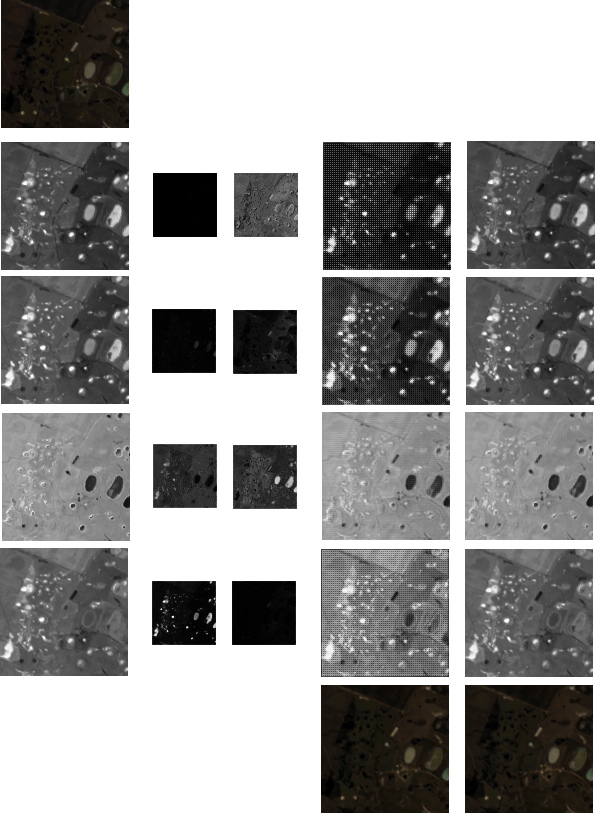
\includegraphics[scale=0.6]{img/latents_2.png}
\caption{Latent image comparison}
\label{fig:latentcompare}
\end{figure}

\begin{figure}
\centering
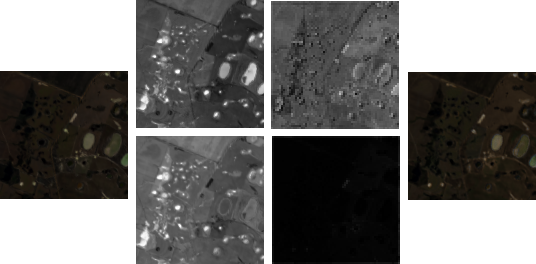
\includegraphics[scale=0.85]{img/innerlatent.png}
\caption{Inner latent comparison}
\label{fig:innerlatent}
\end{figure}

The best performing model for this experiment was \textbf{FastCombined-EncoderFrozen} with $\lambda=0.5$ with a \ac{psnr} of 45.50 dB and a spectral angle of $3.06 \degree$. The second best model was \textbf{FastCombined-AllFrozen} with $\lambda=0.7$ with a \ac{psnr} of 45.31 and a spectral angle of $3.22 \degree$.

\section{Results of Models Using Hyperprior-based Spatial Compression\label{sec:ch5hyperprior}}
\begin{table}
\centering
\begin{tabular}{|c|c|c|c|c|c|c|}
\hline
Model & F & Loss &$\varphi$ & bpppc & PSNR (dB) & Spectral Angle ($\degree$) \\
\hline\hline
CombinedWithAttention & 1 & RD & - & XXX & XXX & XXX \\
\hline
CombinedWithAttention & 1 & MSE & - & XXX & XXX & XXX \\
\hline
CombinedWithAttention & 4 & RD & - & XXX & XXX & XXX \\
\hline
CombinedWithAttention & 4 & MSE & - & XXX & XXX & XXX \\
\hline
CombinedWithAttention & 16 & RD & - & XXX & XXX & XXX \\
\hline
CombinedWithAttention & 16 & MSE & - & XXX & XXX & XXX \\
\hline
CombinedWithAttention & 64 & RD & - & XXX & XXX & XXX \\
\hline
CombinedWithHyperprior & 256 & RD & 0.1 & 1.65 & 19.30 & 24.56 \\
\hline
CombinedWithHyperprior & 256 & MSE & - & 216.35 & 36.80 & 5.79 \\
\hline
Conv1DHyperprior & - & RD & 0.1 & 2.12 & 35.99 & 8.92 \\
\hline
Conv1DHyperprior & - & MSE & - & 96.38 & 34.98 & 9.83 \\
\hline
Attention-Based (\citep{cheng_learned_2020}) & 256 & RD & 0.1 & 0.2446 & 33.92 & 8.71 \\
\hline
Scale Hyperprior (\citep{balle_variational_2018}) & 256 & RD & 0.1 & 2.09 & 20.92 & 24.765 \\
\hline
\end{tabular}
\caption{Comparison of hyperprior models}
\label{fig:hyperpriorcomp}
\end{table}

\section{Kernel size change in 2D CNN-based spatial autoencoder}
\begin{table}
\centering
\begin{tabular}{|c|c|c|c|}
\hline
Kernel Size & Per Channel? & PSNR (dB) & Spectral Angle ($\degree$) \\
\hline\hline
3 & No & \textbf{45.50} & \textbf{3.06} \\
\hline
5 & No & 43.72 & 3.30 \\
\hline
7 & No & 42.59 & 3.58 \\
\hline
3 & Yes & 42.33 & 3.30 \\
\hline
\end{tabular}
\caption{Comparison of different kernel sizes for the spatial autoencoder and per-channel spatial autoencoder with the baseline model. For all models the spectral encoder is frozen after pretraining and $\lambda = 0.5$}
\label{fig:kernelgroups}
\end{table}

To improve the amount of spatial dependencies exploited by the \ac{twod} \ac{cnn}-based spatial autoencoder as part of the Combined Model, we experimented with changing the kernel sizes of the convolutional layers of the spatial autoencoder from three to the higher values five and seven. These experiments were performed using the model \textbf{FastCombined-EncoderFrozen} with $\lambda=0.5$. However, as seen in \autoref{fig:kernelgroups}, this did not improve either \ac{psnr} or spectral angle. The highest metrics were achieved by the base model using a kernel size of three with 45.50 dB and a spectral angle of $3.06 \degree$. The model using a kernel size of five achieved a lower \ac{psnr} of 43.72 dB and a higher spectral angle of $3.30 \degree$, the model using kernel size of seven resulted in the lowest ac{psnr} of 42.59 dB and the lowest spectral angle with $3.58 \degree$. We therefore conclude that a low kernel size of three is optimal for the \ac{cnn}-based spatial autoencoder.

\section{Per-Channel 2D CNN-based spatial autoencoder}
On the HySpecNet-11k dataset, the \ac{jpeg} 2000 baseline performed surprisingly well. \Ac{jpeg} 2000 is executed per channel, therefore performing only spatial compression on 202 single-channel images. However, the \ac{twod} \ac{cnn}-based spatial autoencoder uses the same filters to compress all channels in the bottleneck of the spectral autoencoder. We theorized that the differences between the latent channels might be too large to be appropriately captured using the same filters. 

To test this thesis, we modified the \ac{twod} \ac{cnn}-based spatial autoencoder to use a separate set of filters for each channel in the latent. Since this multiplies the number of parameters by the number of latent channels, we reduced the number of filters per channel. For the layers which originally had 256 filters, the modified model only uses 32 filters. For the layers that originally had 512 filters, the modified model uses 64 filters. The reduction in the number of filters is not only appropriate to reduce the number of parameters for the model, it follows also from the fact that less parameters are required for a convolutional layer that captures dependencies for a single channel than a convolutional layer that captures dependencies for multiple channel simultaneously. In total, the number of parameters in the spatial encoder after the reduction in the number of filters rises by 49.3 \% from 50,849,818 to 75,928,346 parameters. We tested the modified model using the model \textbf{FastCombined-EncoderFrozen} with $\lambda=0.5$. However, the modification did not significantly change the performance of the Combined Model with regard to the metrics \ac{psnr} or the spectral angle as seen in \autoref{fig:kernelgroups}. 

\section{Rate Distortion Comparison\label{sec:ch5heur}}

\begin{figure}[!ht]
\centering
\pgfplotstableread[col sep=semicolon,]{graphs/bitratecomp.csv}\datatable
\begin{tikzpicture}
\begin{semilogxaxis}[
	log ticks with fixed point,
	grid=both,
    width=\textwidth,
    height=10cm,
    xmin=0.05,
    xtick={0,0.05,0.1,0.25,0.5,1,2,4,8},
    %legend style={at={(0.98,0.05)},anchor=south east},
    legend cell align=left,
    legend columns=3,
    legend style={at={(0.5,-0.2)},anchor=north},
    %legend to name={bitratecomplegend},
    ylabel={Psnr},
    xlabel={Bits per pixel per channel},
	cycle list name=color list,
	every axis plot/.append style={mark=o, very thick} % set options for all plots]
	]
    
    \addplot+ table [x={bpppc}, y={psnr}, 
    restrict expr to domain={\thisrow{model_id}}{2:2}]{\datatable};
    \addlegendentry{FastCombined-NF}
    
    \addplot+ table [x={bpppc}, y={psnr}, 
    restrict expr to domain={\thisrow{model_id}}{9:9}]{\datatable};
    \addlegendentry{FastCombined-AF}
    
    \addplot+ table [x={bpppc}, y={psnr}, 
    restrict expr to domain={\thisrow{model_id}}{10:10}]{\datatable};
    \addlegendentry{FastCombined-EF}
    
    \addplot+ table [x={bpppc}, y={psnr}, 
    restrict expr to domain={\thisrow{model_id}}{3:3}]{\datatable};
    \addlegendentry{Conv1D}
    
    \addplot+ table [x={bpppc}, y={psnr}, 
    restrict expr to domain={\thisrow{model_id}}{4:4}]{\datatable};
    \addlegendentry{Combined}
    
    \addplot+ table [x={bpppc}, y={psnr}, 
    restrict expr to domain={\thisrow{model_id}}{5:5}]{\datatable};
    \addlegendentry{FastConv1D}
    
    \addplot+ table [x={for_combined}, y={psnr}, 
    restrict expr to domain={\thisrow{model_id}}{11:11}]{\datatable};
    \addlegendentry{CombinedWithAttention}
    
    \addplot+ table [x={bpppc}, y={psnr}, 
    restrict expr to domain={\thisrow{model_id}}{12:12}]{\datatable};
    \addlegendentry{Conv2D}
    
    \addplot+ table [x={bpppc}, y={psnr}, 
    restrict expr to domain={\thisrow{model_id}}{13:13}]{\datatable};
    \addlegendentry{Spectral-VAE}
    
	\addplot+ table [x={bpppc}, y={psnr}, 
    restrict expr to domain={\thisrow{model_id}}{0:0}]{\datatable};
    \addlegendentry{Cubic Interpolation}
    
    \addplot+ table [x={bpppc}, y={psnr}, 
    restrict expr to domain={\thisrow{model_id}}{1:1}]{\datatable};
    \addlegendentry{Linear Interpolation}    
    
    \addplot+ table [x={bpppc}, y={psnr}, 
    restrict expr to domain={\thisrow{model_id}}{8:8}]{\datatable};
    \addlegendentry{JPEG2000}
    
    \node at (axis cs:0.07,43.4) {0.017};
\end{semilogxaxis}
\end{tikzpicture}
%\ref{bitratecomplegend}
\caption{Rate distortion plot}
\label{fig:ratedistortion}
\end{figure}

Since the distortion produced by a lossy compression method depends on the compression rate \citep{berger_rate-distortion_2003}, we compared the different model architectures used in this thesis for multiple bitrates. We compare all model types listed in \autoref{fig:shortnames} as well as multiple baselines. All learning-based models were trained with a learning rate of $0.5\cdot 10^{-4}$. The models \textbf{Conv1D}, \textbf{FastConv1D} and \textbf{Spectral-VAE} were trained for 70 epochs. The models \textbf{Combined}, \textbf{FastCombined} and \textbf{CombinedWithAttention} were trained for 50 epochs using the corresponding pre-trained spectral autoencoder. The model \textbf{Conv2D} was also trained for 50 epochs. For the model \textbf{FastCombined}, three variations were compared. For \textbf{FastCombined-NF}, the model is trained without freezing either the spectral encoder or decoder after pretraining, for \textbf{FastCombined-EF}, the spectral encoder is frozen after pretraining and for \textbf{FastCombined-AF}, the spectral encoder and decoder are frozen after pretraining. While the differences between these options were already discussed for a fixed bitrate of 0.5 bpppc in \autoref{sec:ch5dualmse}, they are also included in this experiment because of the surprising result that freezing the spectral encoder becomes significantly more important for lower bitrates, as discussed below in this section. The model \textbf{FastCombined-NF} uses \ac{dualmse} loss with $\lambda=0.5$, the models \textbf{FastCombined-EF} and \textbf{FastCombined-AF} use $\lambda=1$. For the models \textbf{Combined} and \textbf{CombinedWithAttention}, the best-performing options were used. For \textbf{Combined}, this is \textbf{EncoderFrozen} with $\lambda=0.5$ and for \textbf{CombinedWithAttention} this is \textbf{AllFrozen} with $\lambda=1$. The models \textbf{Combined} and \textbf{FastCombined} use a spatial compression factor of 4. The highest tested bitrate for such a model is therefore $\frac{1}{4}$ of the highest tested bitrate for the models \textbf{Conv1D} and \textbf{FastConv1D}.

Multiple baselines were used to quantify the performance of the models. The first two baselines, \textbf{Linear Interpolation} and \textbf{Cubic Interpolation} perform simple spectral interpolation. For compression using these methods, a given number of equidistant spectral channels are retained and all others discarded. For decompression the original channels are then restored using either linear or cubic interpolation. The first and last channel are always retained, since otherwise restoration of all channels would be impossible without extrapolating values. These methods were used as baselines because of the assumption that nearby spectral channels have similar values for the same pixel, since they capture wavelengths that are close together. The third baseline used was \ac{jpeg} 2000, which was applied per-channel. The tested quality settings for \ac{jpeg} 2000 were 1, 2, 3, 4, 5, 10, 15 and 20. We also consider \textbf{Conv1D} a baseline, since it is based on the model proposed in Kuester et.al. \citep{kuester_1d-convolutional_2021,kuester_transferability_2022}.

The results show that the model \textbf{Spectral-VAE} is not successful in performing hyperspectral image compression by reducing the number of spectral channels. This is not surprising since the \ac{vae} architecture in \ac{rgb} image compression is also not commonly applied directly but rather through using a hyperprior architecture. A hyperprior-based spectral autoencoder is tested and discussed in \autoref{sec:ch5hyperprior}. All other tested model outperform the interpolation-based baselines, showing that the spectral dependencies are too complex to be captured using only interpolation.

In comparison with the \ac{jpeg} 2000 baseline and the models using the Combined Model architecture, the purely spectral compression methods \textbf{Conv1D} and \textbf{FastConv1D} perform best for bitrates close to 0.5 \ac{bpppc}. The model \textbf{Conv1D} outperforms \ac{jpeg} 2000 for the bitrate 0.63 \ac{bpppc}. Note that different model types can be tested for slightly different bitrates because of different padding strategies. Additionally, \ac{jpeg} 2000 can only be set to a fixed number of different quality settings and therefore does not allow for setting a specific bitrate. The model \textbf{FastConv1D} has a higher \ac{psnr} than \ac{jpeg} 2000 for bitrates from 0.31 to 0.47 \ac{bpppc}. These correspond to two and respectively three channels in the latent representation. For higher bitrates, \ac{jpeg} 2000 outperforms the spectral encoding methods. Further, the model \textbf{Conv1D} has a lower limit on the number of spectral channels in the latent dimensions, below which distortion strongly increases. This point is at 2 latent channels, which corresponds to a bitrate of 0.31 \ac{bpppc}, where it achieves a \ac{psnr} of 20.40 dB, while for 4 latent channels, the model achieves 43.63 dB for a bitrate of 0.63 \ac{bpppc}.

The Combined Model architecture outperforms all baselines and other compared models for bitrates at or below 0.5 \ac{bpppc}. The model \textbf{Combined} has a \ac{psnr} of 43.48 when using 13 latent channels which results in a bitrate of 0.51 \ac{bpppc}. For 26 latent channels, the model does not significantly improve, achieving a \ac{psnr} of 43.85 dB with a bitrate of 1.03 \ac{bpppc}, which is worse than \textbf{Conv1D}, \textbf{FastConv1D} and \ac{jpeg} 2000 for similar bitrates. This is expected, since the idea of the Combined Model architecture is to first reduce the number of spectral channels in order to be able to use spatial compression methods that work best for images with a low number of spectral channels such as \ac{rgb} or multispectral images. This is also illustrated by the model \textbf{Conv2D}, which shows the \ac{twod} \ac{cnn}-based spatial autoencoder directly applied to the hyperspectral data. This model only achieves a \ac{psnr} of 35.734 dB for a bitrate of 0.51 \ac{bpppc}, which shows that a reduction in the amount of channels can strongly improve the performance of spatial compression methods. The effect is further shown by the model \textbf{AttentionHyperprior}, which uses the spatial autoencoder of the \textbf{CombinedWithAttention} model without first reducing the number of spectral channels, achieving a much lower \ac{psnr} of 33.92 dB. The model \textbf{FastCombined-AF} achieves the highest \ac{psnr} of all compared models, 44.59 dB, for the bitrate 0.51. For the bitrates 0.23 \ac{bpppc} and 0.12 \ac{bpppc} it is the second best model behind \textbf{CombinedWithAttention} with \acp{psnr} of 42.35 and 38.98 respectively. However, the model \textbf{FastCombined-NF} performs much worse for the bitrate $0.12$ with only a \ac{psnr} of 20.44 dB. It follows that freezing the spectral encoder is important when training for very low bitrates.

For all bitrates below 0.25, the highest \ac{psnr} is achieved by the model \textbf{CombinedWithAttention}. Additionally, this distortion is achieved with a much lower bitrate than in other models with similar \ac{psnr} values. In comparison with the second model with the second lowest bitrate for similar distortion, \textbf{FastCombined-AF}, the compression rate differs by a factor of $0.24/0.017=14.11$. We conclude that for the HySpecNet-11k the \textbf{CombinedWithAttention} model is optimal in order to achieve bitrates $<0.25$ \ac{bpppc}, while the \textbf{FastCombined} model can achieve slightly lower distortion for bitrates $\approx 0.5$ \ac{bpppc}. Additionally, the results show that the Combined Model approach improves upon both purely spectral and purely spatial compression for bitrates lower than 1 \ac{bpppc}. 





